\documentclass[12pt]{article}
\usepackage[top=0.6in, bottom=0.6in, right=0.7in, left=0.7in,
paperwidth=8.5in, paperheight=11in, nohead]{geometry}
\geometry{letterpaper}
\usepackage[pdftex]{graphicx}
\usepackage{color}
\usepackage[normalem]{ulem}
\usepackage{amssymb}
\usepackage{amsmath}
\usepackage{epstopdf}
\usepackage{setspace}
\usepackage{mdwlist}
\usepackage{verbatim}
\usepackage{tikz}
\usepackage{rotating}
\usepackage[numbers]{natbib}

%% make bibliography more compact \setlength{\bibsep}{0in}
\renewcommand\bibsection{\subsubsection*{\refname}}
\title{Transitioning from JAGS/BUGS to NIMBLE}
\author{L.C.~Ponisio, Perry de Valpine, Nicholas L. Michaud}
\def\code#1{\texttt{#1}}

\begin{document}

\maketitle

\section{Steps}
\begin{enumerate}
\item Wrap your
  JAGS/BUGS model code in \code{nimbleCode(\{\})}, directly in R. This
  replaces the step of generating a file containing the model code, as
  is often done
  via \code{cat} or \code{sink} prior to calling BUGS/JAGS
  via \code{R2WinBUGS}, \code{R2jags},
  \code{rjags} or \code{jagsUI}.  (Alternatively, one can read
  JAGS- and BUGS-formatted code and data files using
  \code{readBUGSmodel}.)
\item Provide information about empty indices.  The easiest solution
  is to write the index range explicitly. For example, \code{Omega[,]} will not work in NIMBLE, but
  \code{Omega[1:nsite,1:nspecies]} will.  (Alternatively, one can use
  the \code{dimensions} argument to \code{nimbleModel}.)
\item Split the \code{data} for BUGS/JAGS into \code{data} and
  \code{constants} for NIMBLE.  Constants are necessary to define the
  model, such as \code{nsite} in \code{for(i in 1:nsite) \{...\}}.  Data are
  observed values of some variables, which in NIMBLE can be changed
  and do not need to be provided when a model is created via
  \code{nimbleModel}.  (Alternatively, one can provide a list of both
  constants and data for the \code{constants} argument to
  \code{nimbleModel}, and NIMBLE will determine which is which.)
\item Convert \code{inits} and \code{monitors} inputs from functions to named lists.
\item To run an MCMC on your model, you have two choices:
  \begin{itemize}
  \item Use \code{nimbleMCMC()} much like a call to
  \code{jags()} from the R2jags package.  This will take all steps to
  set up and run an MCMC using
   NIMBLE's default configuration (Figure \ref{fig:wf}). 
 \item To use NIMBLE's full flexibiilty, build the model, configure
   and build the MCMC, and compile both the model and MCMC before
   running the MCMC. Each of
   these pieces can be customized
  and/or explored individually (Figure \ref{fig:wf}).
  \end{itemize}
\end{enumerate}


\section{Differences}
\begin{enumerate}
\item NIMBLE models allow alternative parameterizations for
  distributions (e.g. \code{sd} instead of \code{tau}), vectorized
  math, and user-defined functions and distributions.  
\item NIMBLE allows an MCMC configuration to be customized by changing
  the the samplers to be used.
\item NIMBLE allows new samplers and other kinds of algorithms to be
  programmed from R.
\item \code{burnin} in NIMBLE is post-thinning -- whereas it is pre-thinning in
  BUGS/JAGS -- when using the \code{runMCMC} function.
\end{enumerate}

\clearpage
\begin{sidewaysfigure}
  \centering
  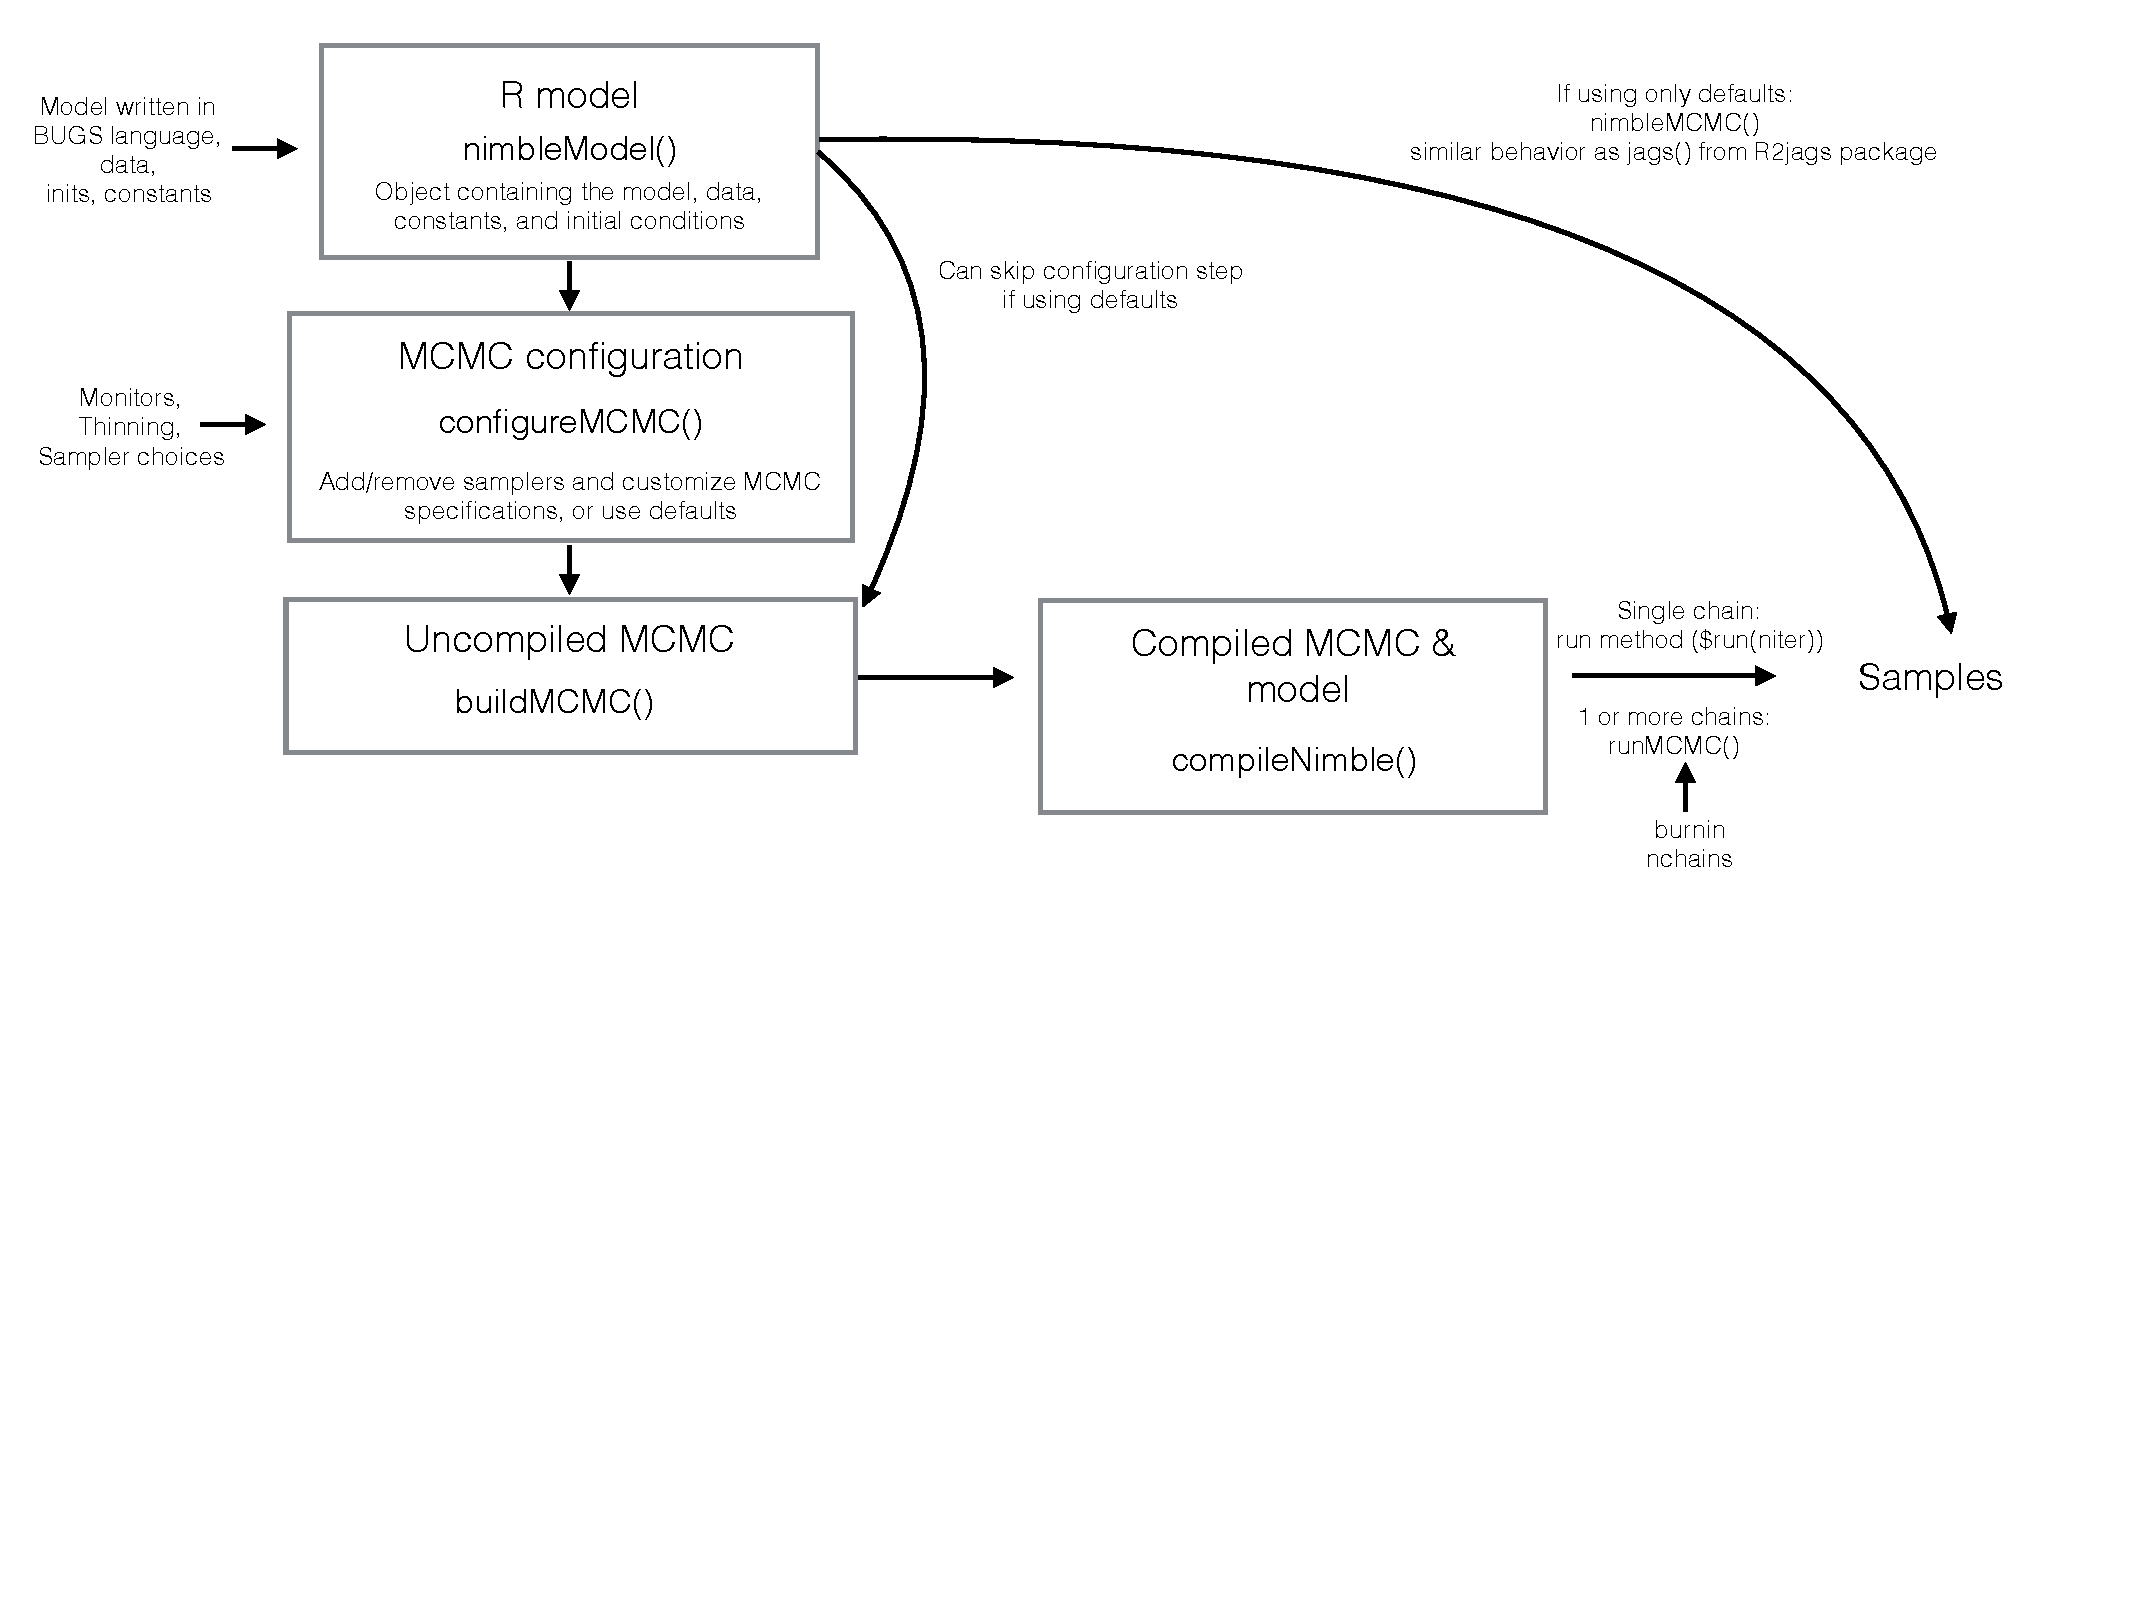
\includegraphics[width=.8\textwidth]{figures/nimbleWorkflow.pdf}
  \caption{Workflow options within NIMBLE.}
  \label{fig:wf}
\end{sidewaysfigure}
\clearpage


\end{document}

%%% Local Variables:
%%% mode: latex
%%% TeX-PDF-mode: t
%%% End:


